% Compiler:     pdflatex

\documentclass[12pt,a4paper]{article}

\usepackage{amsmath, amssymb}
\usepackage[utf8]{inputenc}
\usepackage[english]{babel}
\usepackage{graphicx}
\usepackage[margin=0.5in]{geometry}
\usepackage{float}
\usepackage{subcaption}
\usepackage{caption}

\graphicspath{{fig/}}

\title{MF2007 - Workshop A}

\author{
Adam Lang \\ 861110-3956
\and
Gabriel Andersson Santiago \\ 910706-4538
\and 
Andreas Fr\"oderberg \\ 880730-7577
}

\begin{document}
\maketitle
\section*{Parameter identification}
This section covers the methods behind finding the parameters to enter into the
model to get the biggest similarity to the physical plant
\subsection*{Level 1}
To identify the parameters of the DC motor, firstly an idealized model is
studied theoretically to understand which physical parameters that affect the
performance of the motor. In the Laplace frequency domain, a model of the motor
without inductance can be expressed as 
\begin{equation}
    \label{eq:motormodel}
    X = \frac {k (1 + \frac{1}{Rd})} {s \frac {J_t} { \frac {k^2} {R} + d} + 1}
    U,
\end{equation}
where $X$ is the rotational speed, $U$ is the input voltage, $k$, $R$ and $d$
are the electric motor constant, internal resistance and the viscous friction.
The variable $J_t$ represents the total inertia of the motor and the load. With
the load inertia after a gear with gear ratio $n$, the total inertia is
\begin{equation}
    \label{eq:inertia}
    J_t = J + \frac{J_{load}}{n^2}.
\end{equation}
Here, the load inertia and the inertia of the motor are separated and the motor
inertia from the datasheet is presumed to be correct, leaving only the load
inertia as an unknown.  Now the relations between the motor parameters and the
time performance can be seen. The time constant is given by the term
\begin{equation}
    \label{eq:timeconstant}
    \frac {J_t} { \frac {k^2} {R} + d}
\end{equation}
and as such contains all the parameters of the motor. According to the final
value theorem, the steady state value from a step input is given by setting
$s=0$ and therefore the steady state gain is given by 
\begin{equation}
    \label{eq:steadystate}
    k (1 + \frac{1}{Rd}).
\end{equation}
This contains only one unknown parameter. Therefore, to estimate the viscous
friction parameter $d$, it is suitable to examine and match the steady state
rotational speed of the real system and the model. Since this model contains no
static friction which is probably present in the real system, the test is
conducted at maximum permissable input voltage to minimize the disturbances in
the test data. Since the desired value does not depend on frequency, only a
square wave input is used to simulate steps in both directions. \par
Now that the friction parameter is presumed to be correct and fixed, the time
constant in Equation (\ref{eq:timeconstant}) only has one unknown, the load
inertia. This is estimated from taking the time constant from step inputs,
simulated by a square wave signal. Again, to minimize model disturbances caused
by the static friction present in the real system, the square wave is run at a
full 24 V.\\
The tuning can be seen in Figure~\ref{fig:l1_sq_a24_f016_dtuned} and
Figure~\ref{fig:l1_sq_a24_f016}. In
Figure~\ref{fig:l1_sq_a24_f016_dtuned}, the model been tuned to take the
viscous friction into account.
\begin{figure}[H]
    \centering
    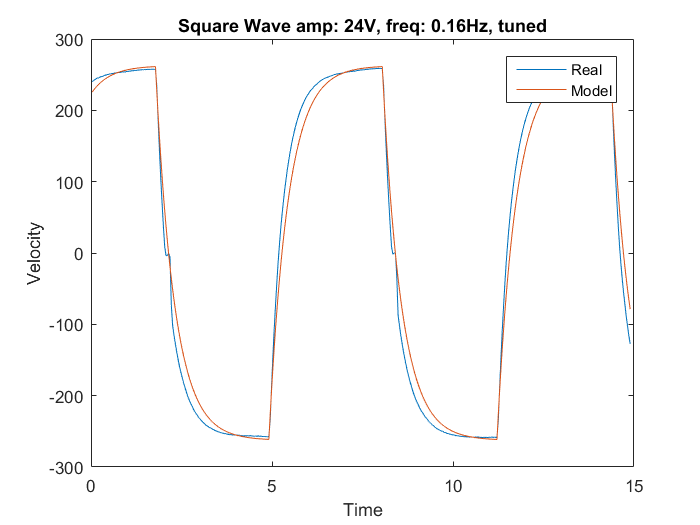
\includegraphics[width=100mm]{l1_sq_a24_f016_dtuned.png}
    \caption{Velocity output from the motor and the model when tuned
t    for viscous friction.}
    \label{fig:l1_sq_a24_f016_dtuned}
\end{figure}
After the viscous friction is modeled, values on the inertia of the
system is adjusted to fit the real motor. The end result after the
parameters have been tuned can be seen in
Figure~\ref{fig:l1_sq_a24_f016}.
\begin{figure}[H]
    \centering
    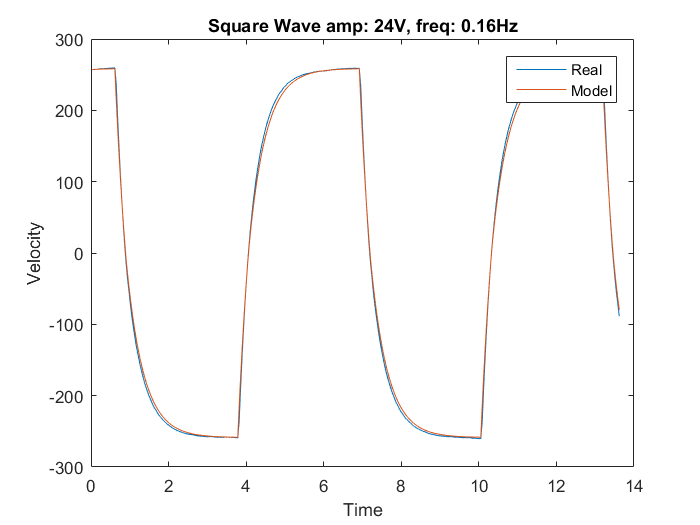
\includegraphics[width=100mm]{l1_sq_a24_f016.png}
    \caption{Velocity output from the motor and the model when tuned for
    both viscous friction and inertia.}
    \label{fig:l1_sq_a24_f016}
\end{figure}

We can clearly see that the model is a much better approximation of the
real motor after the model parameters have been tuned to fit the
real motor. Even though they are not perfect, will the model give a good
sense of the real motor.
\subsection*{Level 2}
\label{sub:level_2}
As could be seen in the earlier friction model, it did not incorporate the
effects of static friction which led to inaccuracy in the model when varying the
rotational speed. A model which captures the real behaviour of the system is
used here, called the Karnop friction model. In addition to the linear friction,
the static friction is taken into account by adding a stick-slip zone where the
friction tourque is equal to the applied torque. The model is given by the
equation
\begin{equation}
    \label{eq:karnop}
    M_f = d \dot{\phi} + F_c sgn(\dot{\phi}),
\end{equation}
with the friction torque $M_f$ and the static friction $F_c$. This
friction is the maximum static friction torque that can be applied in
the stick slip zone.  There is now one more design parameter that needs
to be tuned, $F_c$.  The linear friction is still most prominent when at
high velocities and the static friction is the strongest when at low
velocities. The inertia is decided solely from the rise time and should
not differ much from the previous model.  Firstly, the step response to
a 5 V square wave is examined to determine the static friction. When the
static friction is set, the response to a square wave at 24 V is
examined and $d$ is adjusted to fit the static friction. A sine of low
amplitude is then run to test the behaviour around the stick slip area,
i.e.  at low speeds.\\

In Figure~\ref{fig:l2_sq_a5_f016_fcTuned} the model
have been tuned for static friction. 
\begin{figure}[H]
    \centering
    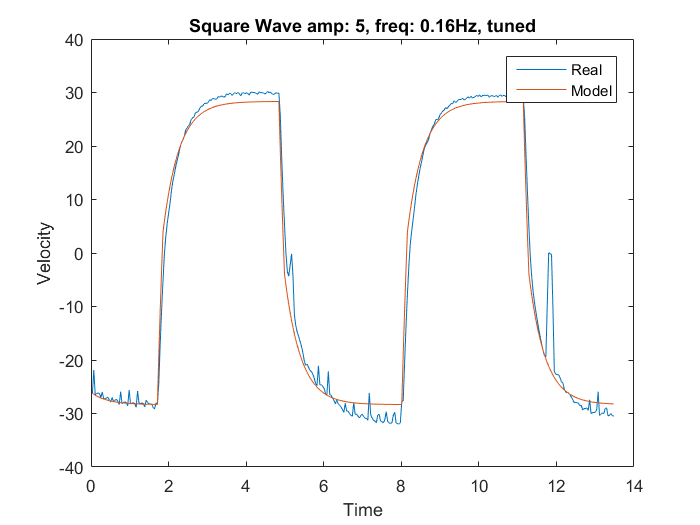
\includegraphics[width=100mm]{l2_sq_a5_f016_fcTuned.png}
    \caption{Velocity response of motor and model at 5V amplitude when
    tuned for static friction.}
    \label{fig:l2_sq_a5_f016_fcTuned}
\end{figure}
In Figure~\ref{fig:l2_sq_a24_f016_fcTuned} the amplitude has been
raised to 24V and the model also have been tuned for static friction.
\begin{figure}[H]
    \centering
    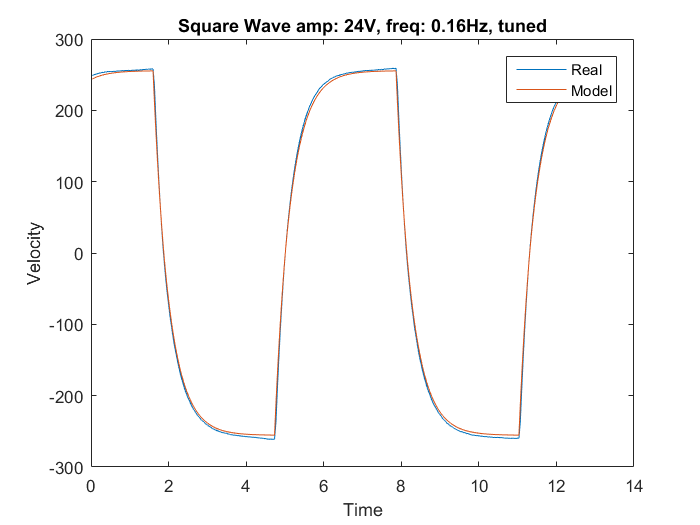
\includegraphics[width=100mm]{l2_sq_a24_f016_fcTuned.png}
    \caption{Velocity response of motor and model at 24V amplitude when
    tuned for both static and dynamic friction.}
    \label{fig:l2_sq_a24_f016_fcTuned}
\end{figure}
After the model have been tuned, is the model compared to the motor when
the input is a 5V sine wave which can be seen in
Figure~\ref{fig:l2_sin_a5_f1}.
\begin{figure}[H]
    \centering
    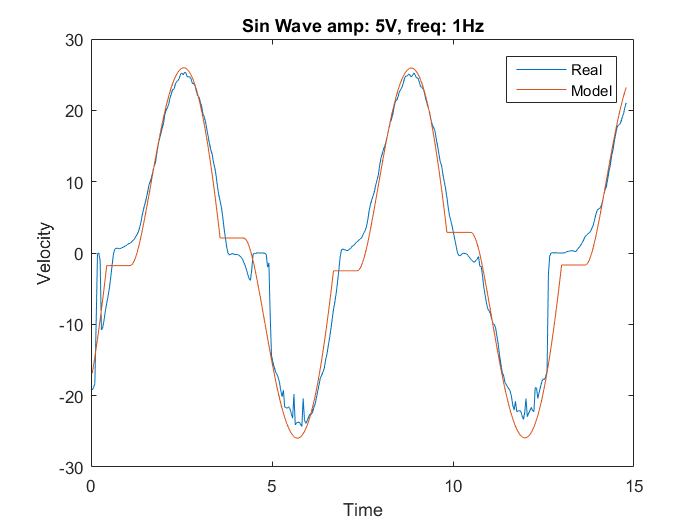
\includegraphics[width=100mm]{l2_sin_a5_f1.png}
    \caption{Velocity response of a sine wave at 5V amplitude of the
    motor and tuned model}
    \label{fig:l2_sin_a5_f1}
\end{figure} 
The lack of a good model for the static friction made the
motor in level 1 be much less accurate when changing the amplitude.
Therefor it had to retuned when a change was made. In level 2 when
introducing the static friction this has now been improved and the model
will now give a much better approximation when changing amplitude.


\section*{Velocity control}
\label{sec:velocity_control}
The parameters generated in the previous section are used to design the
controller for the motor. For the design, a simplified model without motor
inductance is used in \textsc{Matlab} to place the poles and estimate the
behaviour of the system. Furthermore, a non-linear model with Karnop friction is
used in \textsc{Simulink} to simulate the behaviour of the system with the
controller implemented. Finally, the design is run on the actual motor for
verification of plant model and controller.
\subsection*{Level 1}
\label{sub:velocity_level_1}
Controlling the velocity is done with a PI controller. To best control the
performance, the controller is designed in discrete time. \par
The rule of thumb for sample time of a system states that the system should be
sampled at 4-10 times the rise time of the plant in open loop. Using the
simplified model in \textsc{Matlab} and the commando \texttt{stepinfo}, the rise
time is extracted and the sampling time is set to 10 times the rise time. \par
To get the desired performance of the closed loop system, the poles are placed
directly in the discrete plane. First, the plant is converted from continuous to
discrete space by Zero Order Hold (ZOH), with the sampling time derived
earlier.The new sytem matrices are given by the equations
\begin{equation}
    \label{eq:phi}
    \Phi = e^{AT_s}
\end{equation}
and 
\begin{equation}
    \label{eq:gamma}
    \Gamma = \int_0^{T_s}{e^{A(t-s)}B\text{ds}}.
\end{equation}
Output feedback is used to create the closed loop system. 
% Insert figure of output feedback here
The model of the plant is given in (\ref{eq:motormodel}) and is here rewritten as
\begin{equation}
    \label{eq:motorsimple}
    \frac{B}{A}=\frac{a}{s + b}
\end{equation}
,to simplify the equations. 
Firstly, the feedback polynomial $\frac{S}{R}$ is derived. This is given by
\begin{equation}
    \label{eq:feedback_vel}
    \frac{S}{R}=\frac{s_1z + s_0}{z - 1}.
\end{equation}
The system is then closed, yielding the pole polynomial
\begin{equation}
    \label{eq:polepolynomial_vel}
    AR + BS = z^2+(as_1+b-1)z+as_0-b.
\end{equation}
The system is of order one so one closed loop pole given by 
\begin{equation}
    \label{eq:am_vel}
    A_m = z - p_1
\end{equation}
is placed with an additional pole given by the observer polynomial 
\begin{equation}
    \label{eq:ao_vel}
    A_o = z - p_2
\end{equation}
This yields the Diophantine equation
\begin{equation}
    \label{eq:diophantine_vel}
    A_mA_o = AR + BS.
\end{equation}
Solving for (\ref{eq:diophantine_vel}) the unknown controller parameters $s_0$
and $s_1$ are found to be
\begin{equation}
    \label{eq:s0_vel}
    s_0 = \frac{p1p2+b}{a}
\end{equation}
and
\begin{equation}
    \label{eq:s1_vel}
    s_1 = -\frac{b + p_1 + p_2 -1}{a}.
\end{equation}
The $T$ polynomial is given by 
\begin{equation}
    \label{eq:T_vel}
    T = t_0A_o
\end{equation}
where $t_0$ is a static value so that the steady state gain of the closed loop
system is 1. Using the final-value theorem for discrete systems, one yields
\begin{equation}
    \label{eq:t0_vel}
    t0 = \left (\frac{B}{A_m} \right )^{-1}
\end{equation}
evaluated in $z=1$. The control law is then found as,
\begin{equation}
    R(z)u(z)=T(z)r(z)-S(z)y(z)
    \label{eq:contlaw}
\end{equation}
and in numerical form,
\begin{equation}
    (z-1)u(z)=t_0(z-p2)r(z)-(s_1z + s_0)y(z)
\end{equation}


In Figure~\ref{fig:T2_a50_f05:a} is the response from a square wave with
50 rad/s and 0.5Hz shown. In Figure~\ref{fig:T2_a50_f05:b} the voltage
response for the same input is plotted.
\begin{figure}[H]
  \centering
  \begin{subfigure}[b]{0.45\linewidth}
    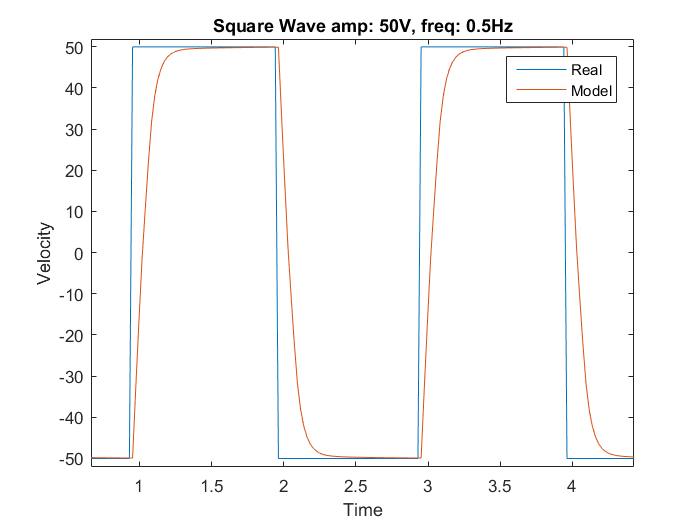
\includegraphics[width=\linewidth]{T2_a50_f05.png}
    \caption{Velocity response }
    \label{fig:T2_a50_f05:a}
  \end{subfigure}
  \begin{subfigure}[b]{0.45\linewidth}
    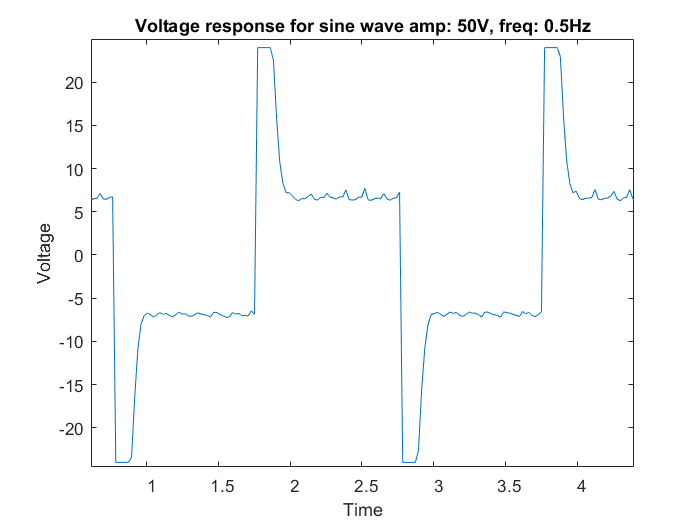
\includegraphics[width=\linewidth]{T2_V_a50_f05.png}
    \caption{Voltage response }
    \label{fig:T2_a50_f05:b}
  \end{subfigure}
  \caption{Response for square wave 50 rad/s and 0.5Hz}
  \label{fig:T2_a50_f05}
\end{figure}
 It can also be seen in
Figure~\ref{fig:T2_a50_f05_ss} the plot that the
steady state error is less than the specified 0.5 rad/s. And that there
is no overshoot.
\begin{figure}[H]
    \centering
    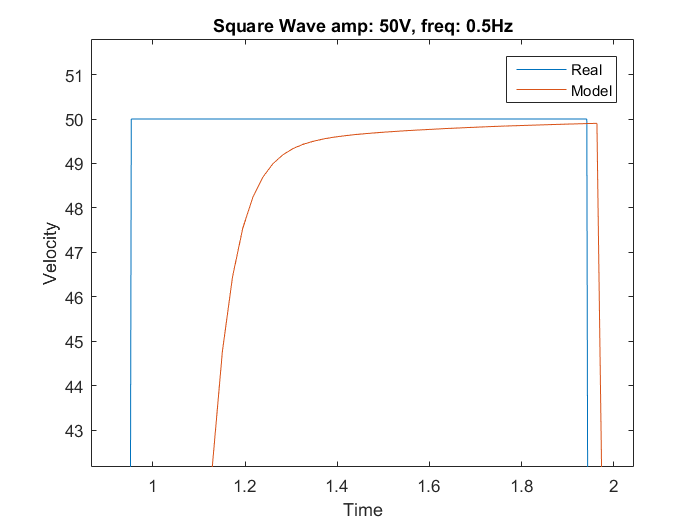
\includegraphics[width=0.45\linewidth]{T2_a50_f05_ss.png}
    \caption{Zoomed plot of the Velocity response}
    \label{fig:T2_a50_f05_ss}
\end{figure}
In Figure~\ref{fig:T2_a10_f02:a} is the response from input of
$\varphi_{ref}=10sin(2\phi 0.2t)$ shown.
\begin{figure}[H]
  \centering
  \begin{subfigure}[b]{0.45\linewidth}
    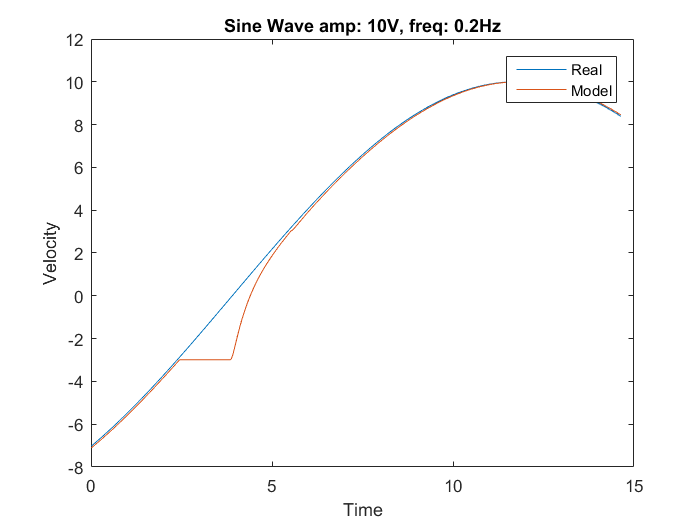
\includegraphics[width=\linewidth]{T2_a10_f02.png}
    \caption{Velocity response }
    \label{fig:T2_a10_f02:a}
  \end{subfigure}
  \begin{subfigure}[b]{0.45\linewidth}
    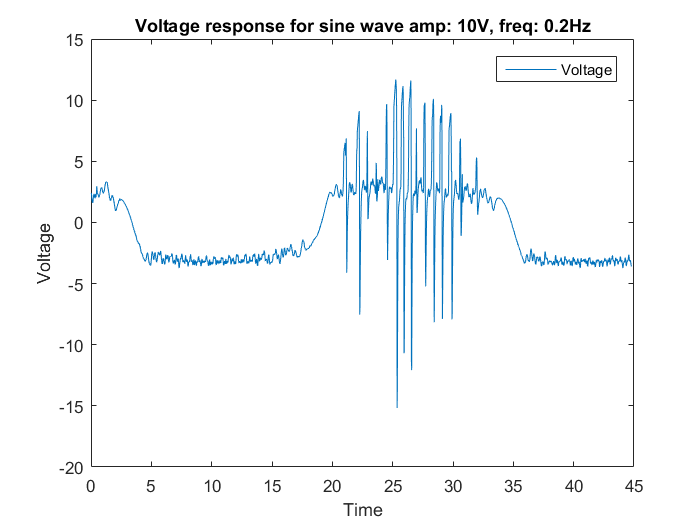
\includegraphics[width=\linewidth]{T2_V_a10_f02.png}
    \caption{Voltage response }
    \label{fig:T2_a10_f02:b}
  \end{subfigure}
  \caption{Response for sine wave 10 rad/s and 0.2Hz}
  \label{fig:T2_a10_f02}
\end{figure}
In Figure~\ref{fig:T2_a10_f02_load:a} is the response from the reference
input of $\varphi_{ref}=10sin(2\pi 0.2t)$ shown. In this plot is the
rotor loaded with a torque by holding it.
\begin{figure}[H]
  \centering
  \begin{subfigure}[b]{0.45\linewidth}
    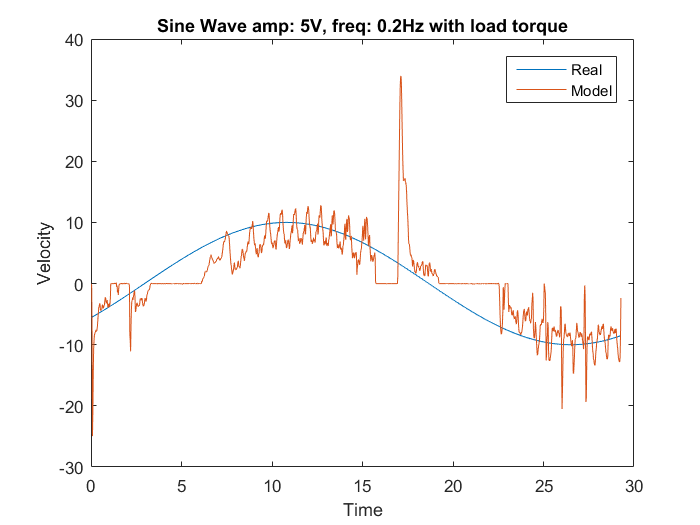
\includegraphics[width=\linewidth]{T2_a10_f02_load.png}
    \caption{Velocity response }
    \label{fig:T2_a10_f02_load:a}
  \end{subfigure}
  \begin{subfigure}[b]{0.45\linewidth}
    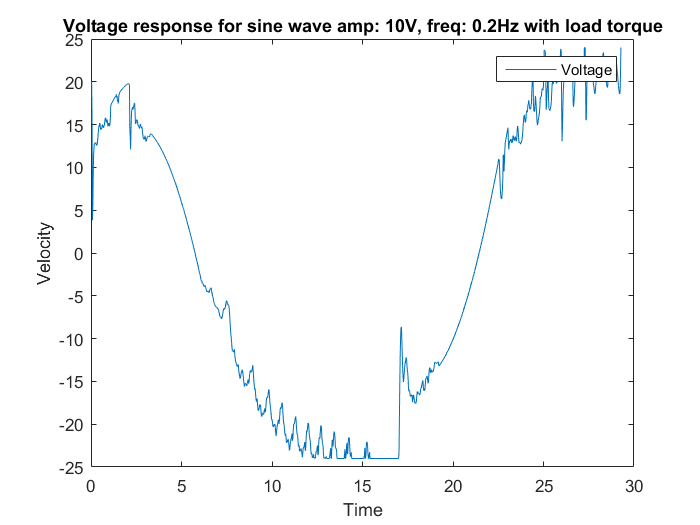
\includegraphics[width=\linewidth]{T2_V_a10_f02_load.png}
    \caption{Voltage response }
    \label{fig:T2_a10_f02_load:b}
  \end{subfigure}
  \caption{Response for sine wave 10 rad/s and 0.2Hz}
  \label{fig:T2_a10_f02_load}
\end{figure}

\section*{Position Control}
  The control law for the position controller is derived similar to the
  velocity controller with the resulting control law in Equation
  \ref{eq:contlaw} as,
  \begin{equation}
      \big((z-1)(z+0.677))u(z)=(71.4z^2-105z+39.9)r(z)-(6.30z^2)y(z)
  \end{equation}
  Where the observer polynomial and the closed loop polynomial is,
  \begin{align*}
        &A_m = (z-0.6)(z-0.5)\\
        &A_o = z^2,
  \end{align*}
  with sampling time $T_s=0.0362$.
  \subsection*{Level 1} 
  In Figure~\ref{fig:pos_cont:a} the response from
  the controller can be seen and in Figure~\ref{fig:pos_cont:b} the
  voltage response is plotted. The specifications is met as can be seen
  in the Figure~\ref{fig:pos_cont:a}
\begin{figure}[H]
  \centering
  \begin{subfigure}[b]{0.45\linewidth}
    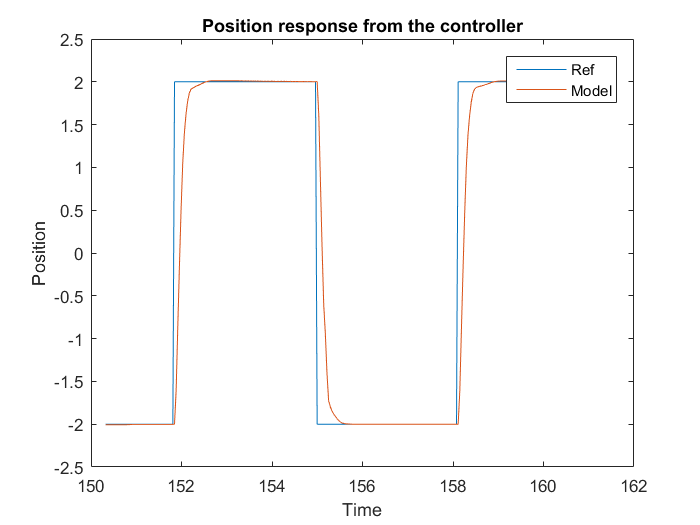
\includegraphics[width=\linewidth]{PosCont.png}
    \caption{Position response}
    \label{fig:pos_cont:a}
  \end{subfigure}
  \begin{subfigure}[b]{0.45\linewidth}
    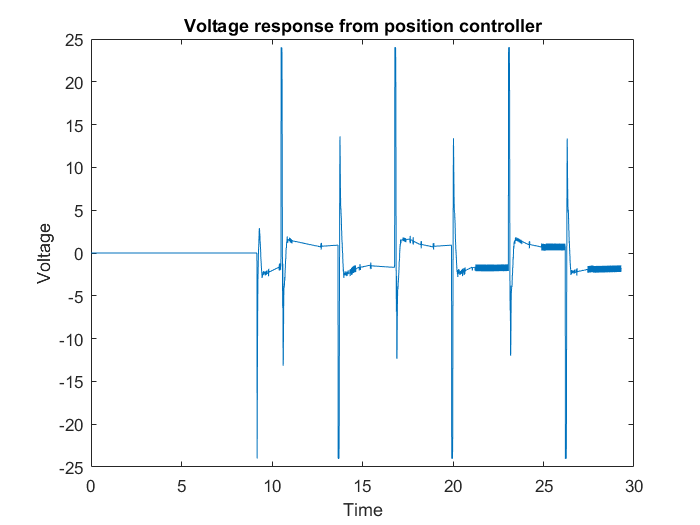
\includegraphics[width=\linewidth]{PosCont_V.png}
    \caption{Voltage response}
    \label{fig:pos_cont:b}
  \end{subfigure}
  \caption{Response from position controller}
  \label{fig:pos_cont}
\end{figure}

\subsection*{Level 2}
The controller used in level 1 is designed directly in the discrete plane. To
compare admissable sampling times, a continuous time controller is designed and
then discretized with Tustins approximation. \par
The design steps are the same as the output feedback design in the velocity
controller case and are therefore not stated again. For the feedback controller,
a continuous PID with low pass filter is chosen,
\begin{equation}
    \label{eq:contpid}
    \frac{S}{R} = \frac{s_2 s^2 + s_1 s + s_0}{s(s+_0)}.
\end{equation}
The Diophantine equation yields the parameter values
\begin{equation}
    \label{eq:r0pos}
    r_0 = 2\omega_3 \zeta - b + \omega_1 + \omega_2, 
\end{equation}
\begin{equation}
    \label{eq:s0pos}
    s_0 = \frac{\omega_1 \omega_2 \omega_3^2}{a},
\end{equation}
\begin{equation}
    \label{eq:s1pos}
    s_1 = \frac{\omega_3 (2\omega_1 \omega_2 \zeta + \omega_1 \omega_3 +
    \omega_2 \omega_3)}{a},
\end{equation}
and
\begin{equation}
    \label{eq:s2pos}
    s_2 = \frac{1}{a} ( -2b\omega_3 \zeta + 2\omega_1 \omega_3 \zeta + 2\omega_2
    \omega_3 \zeta + b^2 - b\omega_2 \omega_1 \omega_2 \omega_3^2),
\end{equation}
where
\begin{equation}
    \label{eq:contpoles}
    A_m A_{o} = (s + \omega_1)(s + \omega_2)(s^2 + 2\omega_3\zeta s +
    \omega_3^2).
\end{equation}
The feedback polynomial becomes
\begin{equation}
    \label{eq:cont_feedback}
    \frac{T}{R} = \frac{t_0 (s^2 + 2\omega_3\zeta s + \omega_3^2)}{s(s + r_0)}.
\end{equation}
Designing the controller is done by iteration and testing. Firstly, the speed
and performance of the system is set by moving the $A_m$ polynomial so that a
good mix of model disturbance and sensor noice rejection is found. The closed
loop poles in $A_o$ are then placed to get the desired performance. The sampling
rate is first set by the thumbrule that it should be 10-30 times faster than the
fastest pole in the system, then it is tuned to see what the maximum reachable
sampling time is while maintaining the perfomance within specifications. The
resultsing control law, sampling time and perfomance is displayed below. \par

\end{document}
